% book.tex -- Copyright (c) 2004, Brian C. Ladd
%
%  Author : Brian C. Ladd 
%  Created: Wed Jul 07 12:03:49 2004 by blad
%  Revised: Fri Dec 28 15:27:43 2007 by blad
%  
\def\FileCreated{Wed Jul 07 12:03:49 2004}
\def\FileRevised{Fri Dec 28 15:27:43 2007}
\documentclass[12pt,oneside]{memoir}
\usepackage{epsfig}
\usepackage{graphicx}
\usepackage[usenames]{color}
\usepackage{xltxtra}
\usepackage{fontspec}
\usepackage{textcomp}
\usepackage{pstricks}
\usepackage{listings}[2000/08/23] 

\usepackage{rotating}
\usepackage{exercise}
% ----- Fonts -----
\defaultfontfeatures{Scale=MatchLowercase,Mapping=tex-text}
\setmainfont{Gentium Book Basic}
\setmonofont{Bitstream Vera Sans Mono}
\setsansfont{Arial}
% ----- Fonts -----

\definecolor{nicered}{rgb}{.647,.129,.149}
\definecolor{listinggray}{gray}{0.1}
\definecolor{templategrey}{gray}{0.85}
\definecolor{NewtonsApple}{gray}{.95}
\definecolor{commandlinebackground}{gray}{.90}
\definecolor{commandlineforeground}{gray}{0.20,}
\definecolor{commandpromptforeground}{gray}{0.55}

\newcommand\code[1]{\lstinline^#1^}
\newcommand\fname[1]{\texttt{#1}}
\newcommand\note[1]{\unskip\footnote{#1}}
\newcommand\foreign[1]{\emph{#1}}
\newcommand\ensurecomma{%
  \@ifnextchar,{}{\@latex@error{Don’t forget the comma!}{}}}
\newcommand\eg{\foreign{e.g.}\ensurecomma}
\newcommand\ie{\foreign{i.e.}\ensurecomma}
\newcommand\cf{\foreign{cf.\@}}

\newcommand\ensuresingleperiod{\@ifnextchar.{}{.\@}}
\newcommand\etc{\foreign{etc}\ensuresingleperiod}
\newcommand\etal{\foreign{et al}\ensuresingleperiod}

\DeclareGraphicsExtensions{.eps,.pdf,.png,.gif,.jpg}

\newcounter{ProgrammingProblem}
\setcounter{ProgrammingProblem}{0}%

\newenvironment{LabExercises}{%
\renewcommand{\ExerciseListName}{Question}%
\renewcommand{\ExerciseListHeader}{\textbf{%
   Checkpoint\ExerciseHeaderNB. }}
\begin{ExerciseList}}%
{\end{ExerciseList}}
\newcommand{\LabExercise}{\Exercise[name={Lab Phase\ExerciseHeaderNB},counter={ProgrammingProblem}]}

\lstset{language=java,
  basicstyle=\small\ttfamily,
  numbers=left, 
  numberstyle=\tiny, 
  stepnumber=1, 
  numbersep=5pt,
  frame=single,
  captionpos=b,
  rulecolor=\color{nicered}
}

\lstdefinelanguage{cline}
{
  morecomment=[s][\color{commandpromptforeground}]{ }{ },
} 

\lstnewenvironment{commandline}[1][]
  {\lstset{language=cline,numbers=none,frame=none,backgroundcolor=\color{commandlinebackground},basicstyle=\color{commandlineforeground},nolol,#1}}
  {}

\setlength{\hoffset}{0in}
\setlength{\voffset}{0in}
\settypeblocksize{9.5in}{7.5in}{*}
\setlrmargins{0.5in}{*}{1}
\setulmargins{0.75in}{*}{*}
\setheadfoot{\onelineskip}{2\onelineskip}
\checkandfixthelayout

\begin{document}

\title{CIS 201 Fall 2008: Lab 7}
\maketitle

\begin{itemize}
\item Implementing a class
\item Using \code{CompositeSprite}
\item Practice using \code{ArrayList}
\item Timed-animation
\item Game components with ``state''
\end{itemize}

\begin{figure}[htb]
  \begin{center}    
    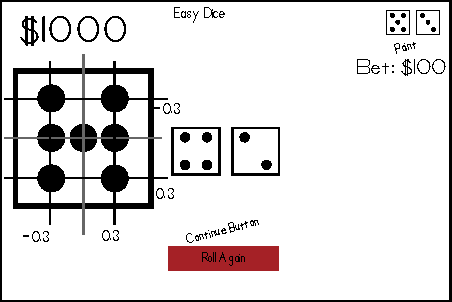
\includegraphics[width=6in]{Drawings/easyDice-design}  
    \caption{EasyDice Design}
  \label{fig:login}
  \end{center}
\end{figure}



\begin{LabExercises}
\LabExercise Download the game \fname{EasyDice.java}. 

Create a directory, \fname{Lab7} in the \fname{CS1} directory. Into
that directory, download the game \fname{EasyDice.java}, available on
Moodle or at
\fname{http://cs.potsdam.edu/faculty/laddbc/Teaching/CS1/EasyDice.java}. 

Look at the contents of the game. It is functional (though you will
have to modify it slightly) \emph{except} that it relies on a class,
\code{OneDie}, that does not exist. Your job, in this lab, is to
create the \code{OneDie} class so that \code{EasyDice} can be played.

Create a new, empty class \code{OneDie}; \code{OneDie} extends
\code{CompositeSprite}. It should be in the same directory as
\fname{EasyDice.java}. Insert a header comment for the file with both
author's names.

Look at the code for \code{EasyDice}. 

In the header comment for \code{OneDie}, write the signature for all
methods called on any object of type \code{OneDie} in the game. You
may want to label these as the interface methods for the class (in the
comment). You know that they must all have \emph{what} access rights?
(Hint: The class \code{EasyDice} must be able to call them from
outside the class \code{OneDie}.)

Don't forget the constructor. It, too, is a method. Include signatures
for any constructors used in \code{EasyDice}.

Before continuing, raise your hand and show the instructors your list
of methods.

\LabExercise Split your list.

Take your list, look at the documentation for \code{CompositeSprite},
and divide your list of methods into two: the first part should be
methods defined in \code{CompositeSprite} or one of its super classes;
the second part, separated by a blank line, should be the methods not
defined in any super class of \code{OneDie}.

You will need to implement the ``new'' methods in your class. You will
extend the \code{CompositeSprite} so you get all of its methods for ``free''.

\LabExercise Implement stubs.

A ``stub'' is a method that doesn't actually do anything. It is used
to permit code to compile while you actually work on getting the code
to function. The stub of a \code{void} method (or a constructor) is
easy: it is empty. There is no need to return any value since none is
expected.

A stub for a method that returns a value just returns some value. For
\code{boolean} you can just return \code{false} and for \code{int} you
can just return \code{0}. You could do the same for \code{double} or
\code{char}. Stubs that are supposed to return objects are a bit
trickier but you don't have any of those here.

Put stubs for all your functions into the \code{OneDie} class and get
\code{EasyDice} to compile. You can run it, too, and you won't see
much.

Show your instructors that you have it compiling.

\LabExercise Change the color and size of the game.
While the game works in the default size of the game, it would work
better if the game were larger. Modify \fname{EasyDice} to have a
default constructor (a constructor with no parameters; this is the
constructor FANG calls) that sets the size of the game to (480, 520)
pixels (the extra height is for the buttons below the play field). 

\LabExercise Add fields

Your dice will need fields. You need to keep track of the value shown
on the die, the game the die is in (for \code{randomInt}), and the
sprites that are the pips and the white background.

As seen in the picture, you will need 7 pips; you can use the
\code{setVisibility} method to turn them on or off depending on the
face that is showing.

\LabExercise Add the sprites.

In the constructor for your dice, you should add eight sprites to
them. The background is a white rectangle, centered at 0, 0 size
1.0. The pips are 0.2 by 0.2 and centered as shown in the
drawing. Note that \code{addSprite} in the \code{CompositeSprite} will
add the sprites. The \code{CompositeSprite} is centered at 0, 0. 

Adding the \code{CompositeSprite} will add all of the sprites you
added to it  to the scene.

\LabExercise Implement get/set for value

Implement \code{setValue}. It should check which number (between 1 and
6) that value is being set to and set the value field \emph{and} turn
on the right pips. You probably want to turn all the pips off first
and then turn on just the ones you want.

Have \code{getValue} return the value set.

\LabExercise Roll the dice.

\code{roll} takes a time parameter, the amount of time you want the
die to roll. It is 2.0 seconds in our case. When I call \code{roll},
change the face (randomly...this is why you need the \code{Game}) and
start counting down. Every eighth to quarter of a second, change the
face. This means you will be running two different countdown timers,
one for the current face and one for the roll.

You will need an \code{advance} method (like the \code{move} method in
\code{BallSprite}) so that the timers can be updated. Your logic will
look like this:

\begin{lstlisting}[numbers=none]
if (animationTimer > 0) {
  // decrement animationTimer
  // decrement faceTimer
  if (faceTimer < 0) {
    // show new random face
    faceTimer = // time to show one face
}

\end{lstlisting}


Also fix up \code{isRolling} to return true so long as there is time
remaining in the current die roll.

\LabExercise Upload Your Java files.

Make sure both authors' names are in all of the header comments!

Go to Moodle; you will find an assignment in week 7 labeled
\textbf{Lab7}. Go there and upload all of the Java files you
created/modified in lab today. Note that there will be other files in
your \fname{Lab7} directory. You want to make sure you upload just the
\fname{.java} file.

\end{LabExercises}


\end{document}

%%% Local Variables: 
%%% mode: latex
%%% End: 

% LocalWords:  Moodle Ladd's login emacs
